\documentclass{beamer}
\usepackage[utf8]{inputenc}
\usepackage[T1]{fontenc}
\usepackage[french]{babel}

\usepackage[export]{adjustbox}
\usepackage{array}
\usepackage{color, colortbl}

\usepackage{graphicx}

\usetheme{JuanLesPins}
\setbeamercolor{structure}{fg=arkred, bg=arkbrown}

% colors
\definecolor{gray73}{gray}{0.73}
\definecolor{arkred}{rgb}{0.592, 0.145, 0.168}
\definecolor{arkbrown}{rgb}{0.239,0.235,0.204}

% template
\setbeamertemplate{blocks}[rounded][shadow=true]
\setbeamercolor{arkblockup}{fg=arkred, bg=arkbrown}
\setbeamercolor{arkblocklow}{fg=white, bg=arkred}

\graphicspath{{../images/}}

\title{Rapport de stage -- Master 2 -- Fiabilité et Sécurité Informatique}
\subtitle{Conception \&  développement système de backup chiffré et
incrémental en C/C++}
\author{Ludovic Lubeigt}
\institute{Aix-Marseille Université}
\date{18 septembre 2015}

\AtBeginSubsection[]
{
  \begin{frame}
  \frametitle{Sommaire}
  \tableofcontents[currentsection, currentsubsection, hideothersubsection]
  \end{frame} 
}

\AtBeginSection[]
{
  \begin{frame}
   \frametitle{Sommaire}
   \tableofcontents[currentsection, hideothersubsection]
  \end{frame}
}

\begin{document}

\begin{frame}
  \begin{minipage}{0.49\textwidth}
    \begin{flushleft}
      \emph{\bfseries Auteur :}\\
      Ludovic \textsc{Lubeigt}
    \end{flushleft}
  \end{minipage}
  \begin{minipage}{0.49\textwidth}
    \begin{flushright}
      
\includegraphics[width=3cm]{logo_sciences.png}
    \end{flushright}
  \end{minipage}\\[2mm]

   
  \begin{beamerboxesrounded}[lower=arkblocklow, shadow=true]{}
    \centering\Large
    Rapport de stage\\ Master 2 -- Fiabilité et Sécurité Informatique\\
    Conception \& développement système de backup chiffré et incrémental en
    C/C++
  \end{beamerboxesrounded}
  
  \begin{figure}[H]
    \begin{minipage}[t]{0.49\textwidth}
      \centering
      
\includegraphics[height=1.4cm]{logo_adhara.png}
    \end{minipage}
    \begin{minipage}[t]{0.49\textwidth}
      \centering
      
\includegraphics[height=1.4cm]{logo_arksens.png}
    \end{minipage}\\[1mm]
  \end{figure}
    
  \begin{minipage}{0.49\textwidth}
    \begin{flushleft}
      \emph{\bfseries Tuteur Entreprise :}\\
      Gaëtan \textsc{van Diemen}
    \end{flushleft}
  \end{minipage}
  \begin{minipage}{0.49\textwidth}
    \begin{flushright}
      \emph{\bfseries Enseignant :}\\
      Jean-Luc \textsc{Massat}
    \end{flushright}
  \end{minipage}\\[1mm]
  
  \begin{center}
    \emph{18 septembre 2015}
  \end{center}
    
\end{frame}

\begin{frame}
 \frametitle{Sommaire}
 \tableofcontents
\end{frame}

\section{Arksens}
\subsection{Présentation de l'entreprise}
\begin{frame}
 \frametitle{Arksens}
 \framesubtitle{Présentation de l'entreprise}
 \begin{minipage}{0.49\textwidth}
  \begin{itemize}
    \item Une présence sur 3 continents
    \item 6 produits
    \item 3 offres clouds
  \end{itemize}
 \end{minipage}
 \begin{minipage}{0.49\textwidth}
  \begin{figure}[h!]
    \centering
    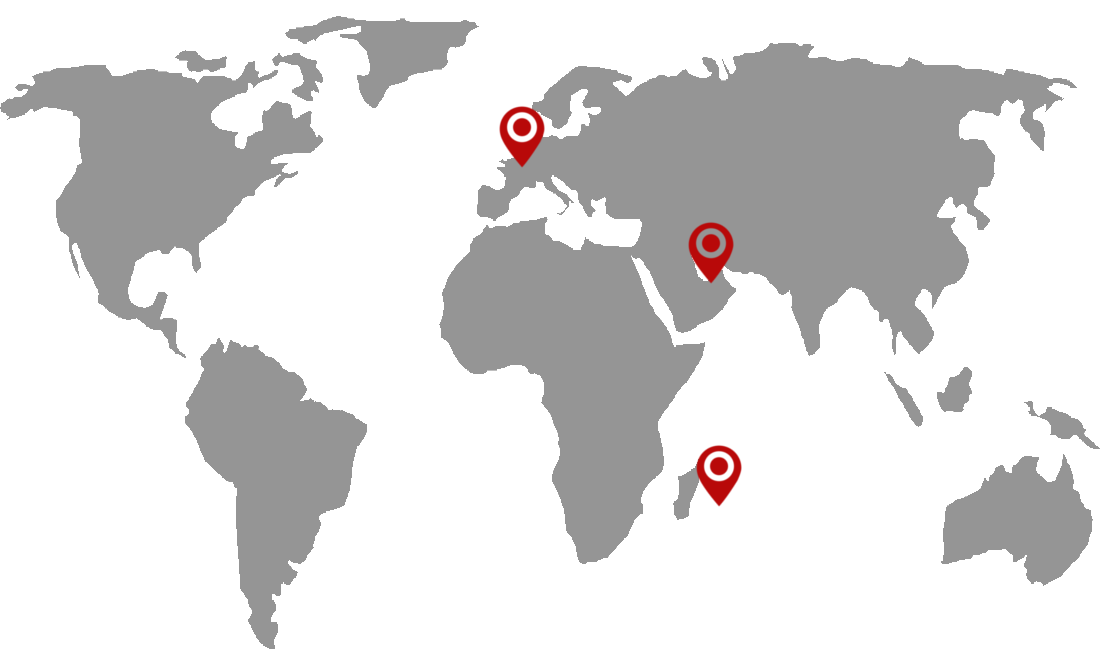
\includegraphics[scale=0.13]{map_arksens.png}
    \caption{Où trouver Arksens ?}
  \end{figure}
 \end{minipage}
\end{frame}

\begin{frame}
  \frametitle{Présentation de l'entreprise}
  \framesubtitle{Les produits et Services}
  \begin{table}[h!]
    \centering
    \def\arraystretch{1.5}
    \setlength{\fboxsep}{13pt} % padding
    \setlength{\fboxrule}{0pt} % frame
    \begin{tabular}{cc}
      \arrayrulecolor{gray73}
      
\includegraphics[width=3cm, fbox]{produits/mail.png} & 
      
\includegraphics[width=3cm, fbox]{produits/whisper.png}\\
      \hline
      
\includegraphics[width=3cm, fbox]{produits/backup.png} &
      
\includegraphics[width=3cm, fbox]{produits/gateway.png}\\
      \hline
      
\includegraphics[width=3cm, fbox]{produits/endpoint.png} &
      
\includegraphics[width=3cm, fbox]{produits/nomad.png}\\
    \end{tabular}
    \caption{Produits et solutions par \textit{Arksens}.}
  \end{table}
\end{frame}

\subsection{Île Maurice}
\begin{frame}
  \frametitle{Présentation de l'entreprise}
  \framesubtitle{Île Maurice}
  \begin{minipage}{0.49\linewidth}
    \begin{itemize}
     \item Recherche et développement
     \item Jusqu'à 8 employés + des commerciaux et le PDG
     \item Importante restructuration
    \end{itemize}
  \end{minipage}
  \begin{minipage}{0.49\linewidth}
    \begin{figure}[h!]
      \centering
      \includegraphics[scale=0.23]{beau_plan_soir.jpg}
      \caption{Beau Plan Business Park.}
    \end{figure}
  \end{minipage}
\end{frame}

\section{Sujet de stage}
\begin{frame}
 \frametitle{Sujet de stage}
 \begin{itemize}
  \item Conception et développement d'un système de sauvegarde 
  chiffré et incrémental
  \item Chiffrement local
  \item Multi-plate-forme
 \end{itemize}
\end{frame}

\section{Déroulement du stage}
\begin{frame}
 \frametitle{Déroulement du stage}
  \begin{minipage}{0.49\textwidth}
    Trois grandes phases
    \begin{itemize}
      \item Recherche
      \item Conception
      \item Développement
    \end{itemize}
  \end{minipage}
  \begin{minipage}{0.49\textwidth}
    \begin{figure}[h!]
      \centering
      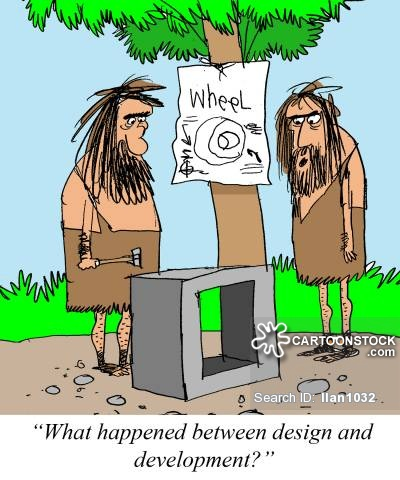
\includegraphics[scale=0.23]{presentation/designAndDevelopment.jpeg}
      \caption{Développement.}
    \end{figure}
  \end{minipage}
\end{frame}

\subsection{Recherche et réflexion}
\begin{frame}
 \frametitle{Recherche et réflexion}
 \framesubtitle{Recherche}
 Des définitions...
 \begin{itemize}
  \item Backup incrémental
  \item Backup différentiel
  \item Transchiffrement\\[0.51cm]
 \end{itemize}
 
 Et des logiciels...
 \begin{itemize}
  \item Syncthing
  \item rsync
 \end{itemize}
\end{frame}

\begin{frame}
 \frametitle{Recherche et réflexion}
 \framesubtitle{Réflexion}
 \begin{itemize}
  \item Chiffrement homomorphique
  \begin{itemize}
   \item Domaine de recherche
   \item Pas utilisable dans des applications aujourd'hui
  \end{itemize}
  \item rsync revisité
  \begin{itemize}
   \item Une base commune avec une fenêtre parcourant le fichier...
   \item ... mais une importante différence avec la taille de la fenêtre
   variant
   \item Un prototype pour valider l'algorithme
  \end{itemize}
 \end{itemize}
\end{frame}

\subsection{Conception}
\begin{frame}
 \frametitle{Conception}
 \framesubtitle{Un programme modulaire}
  \begin{figure}[h!]
    \centering
    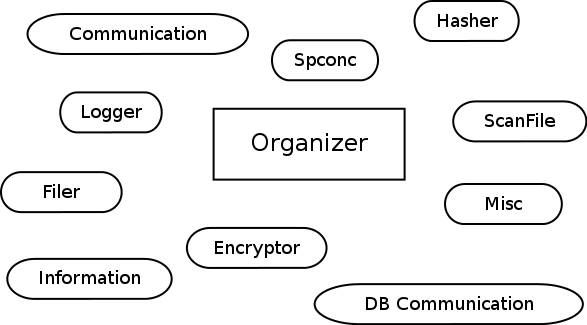
\includegraphics[scale=0.42]{softwareDesign/overviewModule.png}
    \caption{Vue d'ensemble des modules.}
  \end{figure}
\end{frame}

\begin{frame}
 \frametitle{Conception}
 \framesubtitle{Interaction entre modules}
 \begin{minipage}{0.49\textwidth}
  \begin{itemize}
    \item Solution faite maison
    \item Design pattern
    \begin{itemize}
    \item Observer
    \item Event notifier
    \end{itemize}
  \end{itemize}
 \end{minipage}
 \begin{minipage}{0.49\textwidth}
  \begin{figure}[h!]
    \centering
    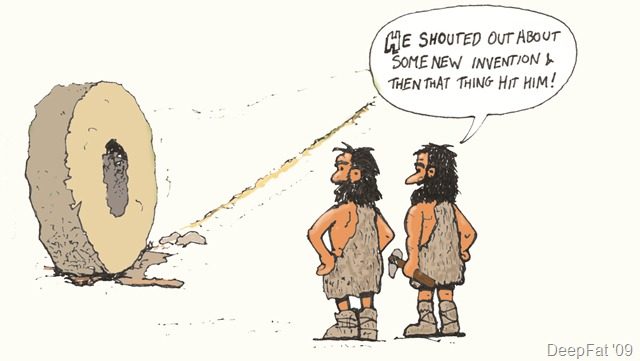
\includegraphics[scale=0.31]{presentation/new_invention.jpeg}
    \caption{Réinventer la roue\footnotemark.}
  \end{figure}
 \end{minipage}
 \footnotetext{Source : \url{http://www.gymmomentum.com/weekly-momentum/
 reinventing-the-wheel-in-gymnastics/}}
\end{frame}

\begin{frame}
 \frametitle{Interaction entre modules}
 \framesubtitle{Event Notifier}
  \begin{figure}
    \centering
    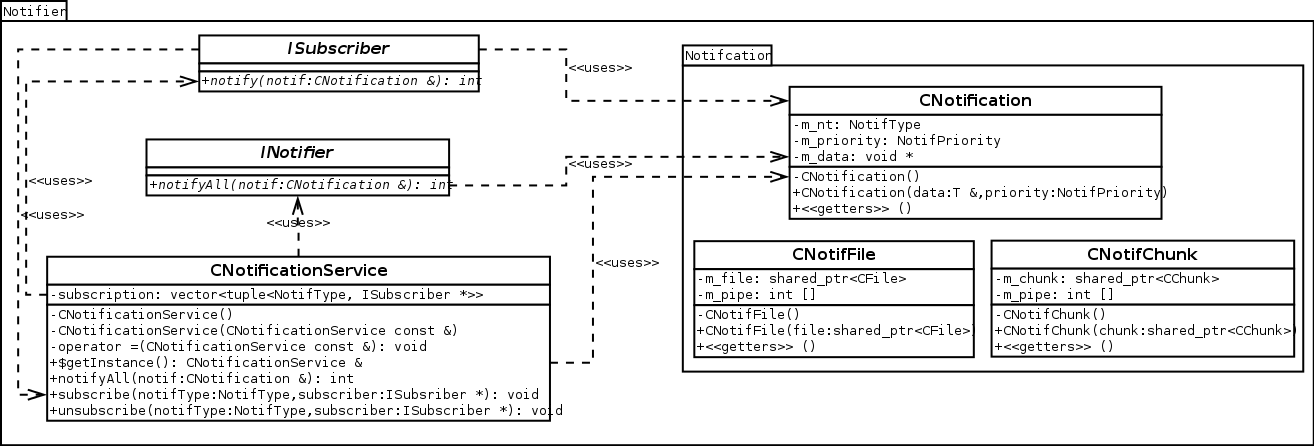
\includegraphics[width=10cm]{softwareDesign/classDiagramNotif.png}
    \caption{Diagramme de classe --- Notifications.}
  \end{figure}
\end{frame}

\begin{frame}
 \frametitle{Interaction entre modules}
 \framesubtitle{Première sauvegarde}
  \begin{figure}
    \centering
    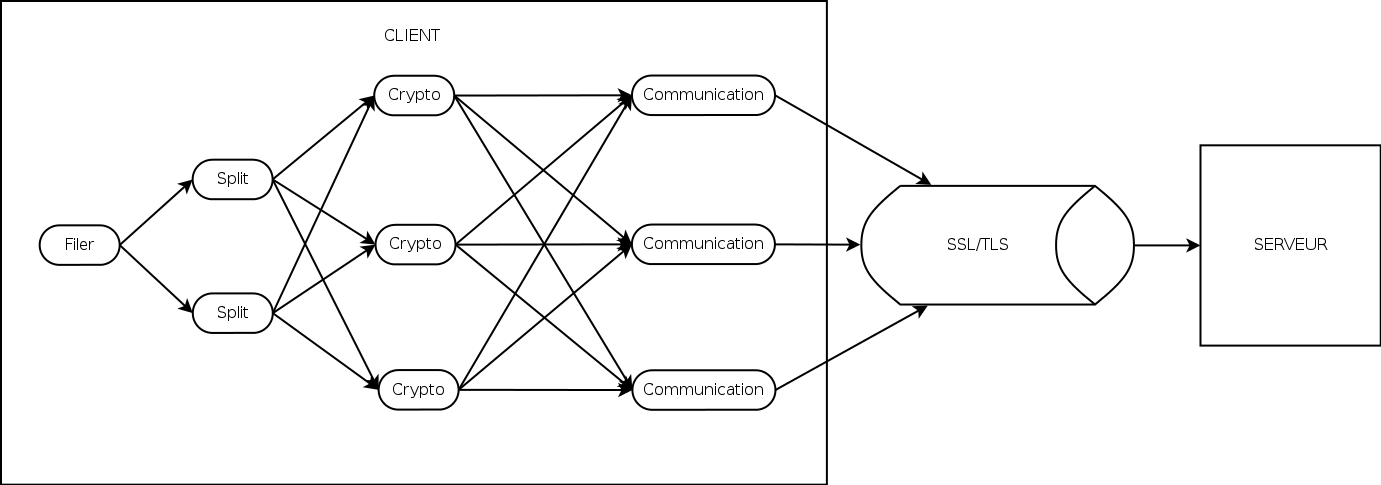
\includegraphics[width=10cm]{softwareDesign/moduleInteraction.png}
    \caption{Fonctionnement lors d'une première sauvegarde.}
  \end{figure}
\end{frame}

\begin{frame}
 \frametitle{Conception}
 \framesubtitle{Base de données}
 \begin{itemize}
  \item Sauvegarder les méta-données de tous les fichiers
  \item Sur le serveur
  \begin{itemize}
   \item Garder une trace de toutes les sauvegardes
   \item Restaurer un fichier à partir de n'importe quelle sauvegarde
  \end{itemize}
  \item Sur le client
  \begin{itemize}
   \item Garder une trace de la dernière sauvegarde
   \item Gain de temps
   \item Économiser de la bande passante
  \end{itemize}
 \end{itemize}
\end{frame}

\begin{frame}
 \frametitle{Base de données}
 \framesubtitle{SQL vs NoSQL}
 \begin{table}[h!]
  \def\arraystretch{1.5}
  \setlength{\fboxsep}{13pt} % padding
  \setlength{\fboxrule}{0pt} % frame
  \begin{tabular}{m{2cm}m{4cm}m{4cm}}
   \rowcolor{arkred} 
    \arrayrulecolor{gray73}\hline
    & \color{white} \textbf{\textit{SQL}} &
    \color{white} \textbf{\textit{NoSQL}}\\
    Stockage des données & Modèle relationnel & Variable : documents,
    clé-valeur, graphe, etc.\\
    \hline
    Schéma et flexibilité & Schéma fixe & Schémas dynamiques\\
    \hline
    Adaptabilité & Évolutivité verticale & Évolutivité horizontale\\
    \hline
    Propriétés ACID\footnote{Atomicité, Cohérence, Isolation,
    Durabilité} & Oui & Pas nécessairement\\
  \end{tabular}
  \caption{\label{tabSQLNoSQL} Tableau comparatif \textit{SQL} et
  \textit{NoSQl}.}
\end{table}
\end{frame}

\begin{frame}
 \frametitle{Conception}
 \framesubtitle{Stockage des données}
  \begin{figure}
    \centering
    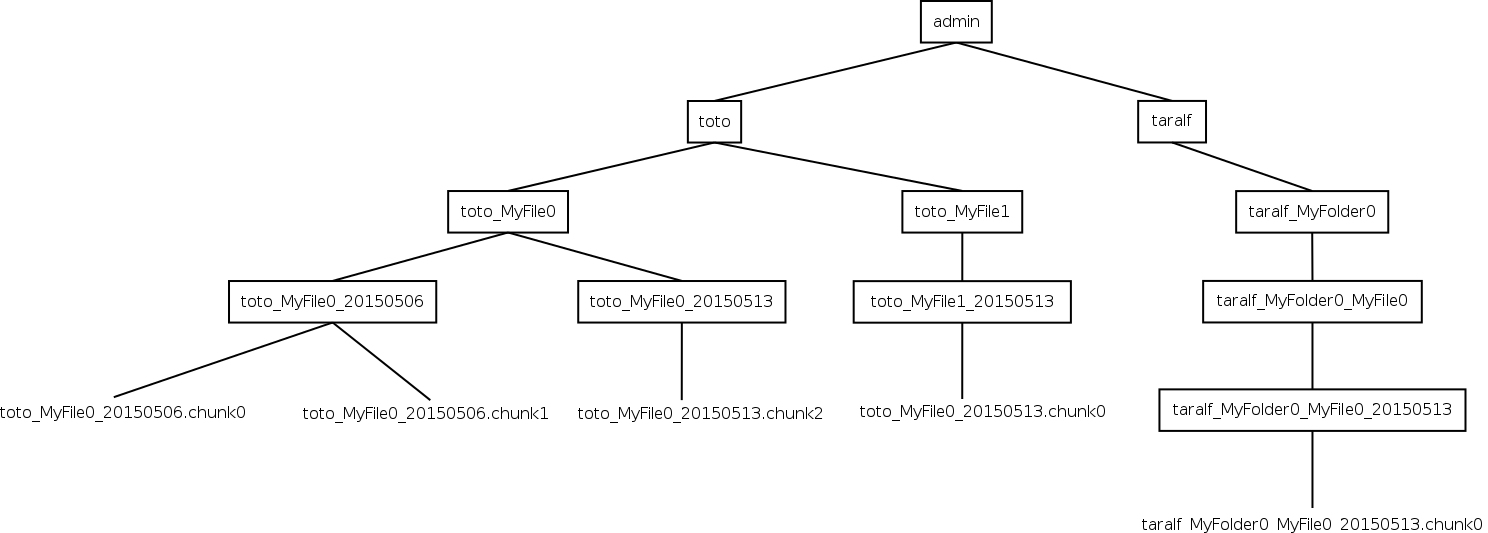
\includegraphics[width=10cm]{softwareDesign/fileSystemServer.png}
    \caption{Stockage des fichiers sur le serveur.}
  \end{figure}
\end{frame}

\subsection{Développement}
\begin{frame}
 \frametitle{Développement}
 \begin{minipage}{0.49\textwidth}
  \begin{itemize}
    \item Utilisation de logiciels, librairies et autres outils de développement
    libres
    \item Module par module
  \end{itemize}
 \end{minipage}
 \begin{minipage}{0.49\textwidth}
   \begin{figure}[h!]
     \centering
     
\includegraphics[scale=0.31]{presentation/logo_opensource.png}
     \caption{Open Source Initiative.}
   \end{figure}
 \end{minipage}
\end{frame}

\begin{frame}
 \frametitle{Développement}
 \framesubtitle{Travail réalisé}
 \begin{itemize}
  \item Développement du client
  \item Modules permettant l'exécution d'une première sauvegarde
  (complète)
  \item Tests unitaires pour chaque module
 \end{itemize}
\end{frame}

\begin{frame}
 \frametitle{Développement}
 \framesubtitle{Problèmes rencontrés}
 \begin{minipage}{0.49\textwidth}
  \begin{itemize}
    \item Chiffrement et déchiffrement
    \item Gestion de la mémoire
  \end{itemize}
 \end{minipage}
 \begin{minipage}{0.49\textwidth}
   \begin{figure}[h!]
     \centering
     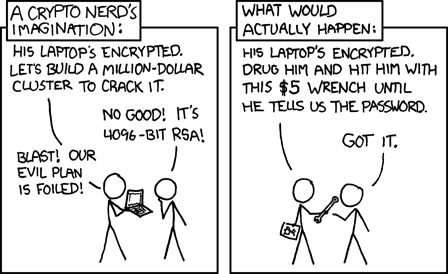
\includegraphics[scale=0.31]{presentation/xkcd_security.png}
     \caption{Sécurité\footnotemark.}
   \end{figure}
 \end{minipage}
 \footnotetext{Source : \url{https://xkcd.com/538/}}
\end{frame}

\section{Conclusion}
\begin{frame}
 \frametitle{Conclusion}
 \begin{itemize}
  \item Première partie du cycle de vie d'un produit
  \item Expérience professionnelle 
  \item Vie dans une startup
 \end{itemize}
\end{frame}


\section*{Questions}
\begin{frame}
\frametitle{Questions}
 \begin{minipage}{0.4\textwidth}
  \begin{center}
    Questions ?
  \end{center}
 \end{minipage}
 \begin{minipage}{0.4\textwidth}
   \begin{figure}[h!]
     \centering
     
\includegraphics[scale=0.37]{presentation/questionmark_cat.jpg}
   \end{figure}
 \end{minipage}
\end{frame}

\section*{Remerciements}
\begin{frame}
 \frametitle{Remerciements}
 Merci de votre attention !
\end{frame}


\end{document}